%A pointform description of the general idea
%\begin{itemize}
%	\item A D-NURBS approach to simulation. Use a Jacobian to map from UV positions in a NURBS parametric space to world space positions on the surface. 
%	\item \textbf{Shape Matching}: From the sample world space positions on a single NURBS surface, we solve a least squares problem to fit a \textit{projection operator} to the surface. This projection operator maps monomials in the undeformed space, to the least squares estimate of the deformed positions for the given monomials.
%	\item With DNURBS and Shape Matching VEM we have two mappings: a UV to undeformed world space with our NURBS Jacobian, then an undeformed to deformed mapping with the projection operators. This lets us form a set of generalized coordinates in terms of our control points of the NURBS surface (section 1.4).
%	\item For an arbitrary position in space (not necessarily on the surface), we can build a projection operator unique to this point via a weighted sum of the projection operators of the projection operators for each NURBS (eq 5). From this we can reconstruct an estimate of the deformed position from the monomial basis defined using its undeformed position.
%	\item For any point in space, we need to compute a set of weights to the projection operators defined on the surfaces with the following criteria: the weights sum to 1, are nonzero, and depend on the distances to the surfaces (See section 1.8).
%	\item With this mapping for undeformed to deformed positions, this yields a simple definition for the deformation gradient (eq 12).
%	\item Armed with our deformation gradient, we next define the Lagrangian, but this basic form isn't sufficient. We augment our kinetic and potential energies with a stability term (ref VEM). This accounts for cases in which the position of the nodal values don't match their estimated positions defined by the projection operator mapping.
%	\item \textbf{Raycasting Quadrature}: To compute the volume integrals we make use of raycasting quadrature approach (ref) where we uniform sample a YZ grid and shoot rays in the X direction. We then use the points of intersection to define integrations bounds for 1D integrals along these rays, which we integrate numerically.
%	\item With our augmented lagrangian, we use the Euler-Lagrange equation to arrive at equations of motion. Our generalized coordinates give us direct updates on the control points of the NURBS. Currently we are using linearly-implicit Euler for time integration.
%	\item \textbf{Handling trimmed NURBS}: For this case we update the original control points, but we must only sample points within the boundary. To compute these points we use an approach similar to the raycasting quadrature but in 2D. In the paremtric domain for a T-NURBS we sample uniforly in the V direction and shoot rays along the U axis. At each region of intersection, we sample more values along the ray. The final result is a set of UV coordinates that respect the boundary defined by NURBS curves.
%\end{itemize}
\section{Overview}
The input to the Shape Matching Element Method (SEM)  is a NURBS \emph{boundary representation} of a volumetric object, along with a set of physical parameters 
(density, constitutive model, model parameters etc). 
The boundary representation is composed of one or more (not necessarily explicit;y connected) NURBS surface primitives that we will call \emph{parts}.
The output is an elastodynamic simulation. 
SEM consists of preprocessing and runtime simulation phases~\refalg{sem} and at no point do we need to generate a volumetric mesh of the input. 
In the \emph{preprocessing} stage we use raycasting to find quadrature points and weights for volumetric integration, as well as to compute part blending parameters. 
Finally we construct local shape matching operators and construct the mass matrix for our problem. 

At runtime we use standard time integration schemes to time step the system (we show linearly implicit, fully implicit, runge-kutta four). 
These require us to evaluate the energy, gradient and Hessian (implicit only) which we do at the previously computed quadrature points. 
For collisions we use penalty forces and apply them as external forces during integration.

\begin{algorithm}[h]
    \label{alg:sem}
    \SetAlgoLined
    \KwResult{Write here the result }
     initialization\;
     \While{While condition}{
      instructions\;
      \eIf{condition}{
       instructions1\;
       instructions2\;
       }{
       instructions3\;
      }
     }
     \caption{Shape Matching Element Algorithm}
    \end{algorithm}

\section{Methods}

Our algorithm acts on objects composed of multiple NURBS surfaces~\reffig{NURBS}.

\begin{figure}
    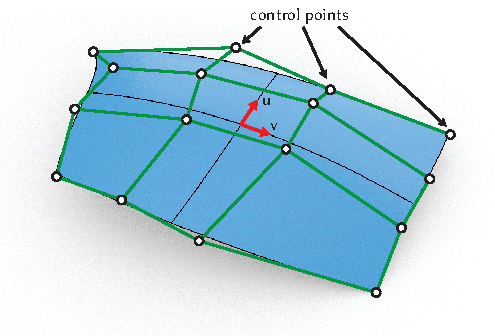
\includegraphics[width=\columnwidth]{figures/nurbs_patch}
    \caption{A cubic NURBS patch with 16 control points.}
    \label{fig:NURBS}
\end{figure}

The three-dimensional position, $\defX$, of any point on a NURBS surface can be written as 
\begin{equation}
\label{eqn:nurbs_srf}
\defX\left(u,v\right) = \sum_{i=1}^n\sum_{j=1}^n \phi_{ij}\left(u,v\right)\vc{q}_{ij},
    %\mathbf{x}(u,v) = \frac{\sum_{i=1}^{n}\sum_{j=1}^{m}  \mathbf{p}_{i,j} w_{i,j} B_{i,k}(u)B_{j,l}(v)}
    %{\sum_{i=1}^{n}\sum_{j=1}^{m} w_{i,j} B_{i,k}(u)B_{j,l}(v)}
    %\text{,}
\end{equation}
where $u$ and $v$ $\in \real$ are the coordinates of the 2D parametric domain, $n$ and $m$ are the number of control points in the $u$ and $v$ directions, $\mathbf{q}_{ij}\in\real^3$ are the control points and $\phi_{ij}\left(u,v\right)\in\real$ are the NURBS
basis functions given by 
\begin{equation*}
    \phi_{ij}\left(u,v\right) = \frac{w_{i,j}B_{ik}(u)B_{jl}(v)}{\sum_{r=1}^{n}\sum_{s=1}^{m} w_{ij} B_{ik}(u)B_{jl}(v)},
\end{equation*} where $B_{ik}$ (resp $B_{jl}$) is the $i^{th}$ ($j^{th}$) b-spline basis of order $k$ ($l$). 

Exploiting linearity with respect to the control points  we can express this mapping as 
\begin{equation}
    \defX\left(u,v\right) = \underbrace{\begin{pmatrix} \phi_{11}\left(u,v\right)\ident & \dots & \phi_{nn}\left(u,v\right)\ident \end{pmatrix}}_{\Jnurbs\left(u,v\right)}
    \underbrace{\begin{pmatrix} \vc{q}_{11} \\ \vdots \\ \vc{q}_{nn}\end{pmatrix}}_{\vc{q}},
\end{equation} where $\Jnurbs\left(u,v\right)$ is the NURBS Jacobian, $\ident$ is the $3\times3$ identity matrix and $\vc{q}$ is the vector of generalized coordinates~\dave{cite Lanczos}.
The Shape Matching Element Method will follow from this kinematic description.

\subsection{Shape Matching}
\label{sec:shapematching}

We begin by describing shape matching to a single NURBS part. 
Given a two different configurations of the same part (specified by the control points), shape matching computes a polynomial deformation which best aligns them.

Let $\vc{q^0}$ be the initial control points of the part, provided by the modeller and Let $\vc{q}$ be a vector of modified control point values.
We can compute the undeformed (or reference) position of any point on our part using $\refX\left(u,v\right) = \Jnurbs\left(u,v\right)\mathbf{q^0}$ and the corresponding
deformed (world space) position as $\defX\left(u,v\right) = \Jnurbs\left(u,v\right)\mathbf{q}$.

We can define a polynomial deformation from $\refX = \begin{pmatrix} X & Y & Z \end{pmatrix}^T$ to $\defX$  as 
\begin{equation}
    \defX\left(\refX\right) = 
    \underbrace{\begin{pmatrix}
    \mathbf{p}^T(\refX-\bar{\refX}) & \mathbf{0} & \mathbf{0} & 1 & 0 & 0\\
    \mathbf{0} & \mathbf{p}^T(\refX-\bar{\refX}) & \mathbf{0} & 0 & 1 & 0\\
    \mathbf{0} & \mathbf{0} & \mathbf{p}^T(\refX-\bar{\refX}) & 0 & 0 & 1\\
    \end{pmatrix}}_{\Pmatx}
    \Pcox,
    \label{eq:projection}
\end{equation} where $\mathbf{p}^T\left(\refX\right)$ is the polynomial basis vector \newline (eg $\begin{pmatrix} X & Y & X\cdot Y & X\cdot X & Y\cdot Y \end{pmatrix}$ ),
$\bar{\refX}$ is an a priori chosen origin around which to deform, $\Pco$ are the coefficients for the 
non-constant part of the polynomial and $\tr$ is the translation of the deformation origin. 
We can compute the shape matching deformation by solving~\cite{10.1145/1073204.1073216}
\begin{equation}
   \Pcox^* = \arg\min_{\Pco,\tr} \int \left\lvert\left\lvert\Pmatx\Pcox - \Jnurbs\vc{q}\right\rvert\right\rvert^2_2 dudv,
\end{equation} where we have suppressed the dependence of $\refX$ and $\Jnurbs$ on $u$ and $v$ for the sake of brevity.

\dave{Ty: need some text to explain how we pick points on the nurbs surface.}
We discretize the shape matching energy and minimize by solving
\begin{equation}
\samp{\Pmat}^T\wt\samp{\Pmat}\Pcox = \samp{\Pmat}^T\wt\samp{\Jnurbs}\vc{q}.
\label{eq:shapematch}
\end{equation} Here $\samp{\Pmat}$ (resp. $\samp{\Jnurbs}$) is a $3s \times 3k$ (resp. $3s \times 3nm$) matrix where $s$ is the number of quadrature points, 
$k$ is the number of  terms in the shape matching polynomial and $3nm$ is the number of NURBS control points. 
$\samp{\Pmat}$ (resp. $\samp{\Jnurbs}$) is constructed by stacking the evaluations of $\Pmatxuv$ (resp. $\Jnurbs\left(u, v\right)$) at each
quadrature point.
$\wt$ is a diagonal, $3s \times 3s$ matrix of integration weights.

\paragraph*{Relationship to the Virtual Element Method}
For a non-planar NURBS part, and given a sufficient number of quadrature points, ~\refeq{shapematch} will be well-posed allowing us to write: $\Pcox^* = \Pi\vc{q}$ where
\begin{equation*}
    \Pi = \left(\samp{\Pmat}^T\wt\samp{\Pmat}\right)^{-1}\samp{\Pmat}^T\wt\samp{\Jnurbs},
\end{equation*} is a projection from the space of control points onto the space of polynomials. 
This projection serves an identical purpose (and is mathematically equivalent up to choice of metric) to the projection operator used in VEM~\cite{10.1142/S021820251440003X}.
VEM uses a single polynomial projection per polyhedral element to solve differential equations on complex volumetric meshes.
We interpret shape matching as converting our NURBS part into a single Virtual Element suitable for elastodynamics simulation.
Unfortunately a single polynomial deformation space will not be suitably expressive for even moderately complex models. 
Previous work~\cite{10.1145/1073204.1073216,10.1145/1275808.1276480} used additional lattices or partitions of the reference space to 
increase the number of polynomials in the shape matching. Next we outline our meshless Shape Element Method which works directly on the NURBS
geometry itself.

\subsection{Shape Matching Element Method}
 Each input object is composed of a set of boundary representations, $\Prts$, one for each part $\prt\in\Prts$. 
 Our kinematic mapping is a blended construction (as is done for skinning~\cite{10.1145/2614028.2615427}) which we write as

 \begin{equation}
    \defX\left(\refX\right) = \sum_{\prt_i\in\Prts} \bld_i\Pmatxi\Pi_i\vc{q}_i, 
 \end{equation} where $w_i$ $\Pmatx_i$, $\Pi_i$ and $\vc{q}_i$ are the blending weights, polynomial basis, projection operator and control points for the $i^{th}$
 part respectively.  
 
 \subsubsection*{Multiple Part Projection}
As in ~\refsec{shapematching} we construct each $\Pi_i$ via shape matching. 
It is tempting to use an identical polynomial basis matrix, $\Pmatx$ for all parts, $\prt_i$, but recall that constructing $\Pmatx$ requires the selection of a deformation
origin $\bar{\refX}$~(\refeq{projection}). 
Using the same origin for all polynomials limits the expressivity of the kinematic model~\cite{STBS:2011}.
Instead we choose a number of points in $\refX$ ($|\Prts| > |\XBs| > 0$, where $\XBs$ is the set of points)  to act as deformation origins~(\refsec{origins}).
For each part we now construct $\Pmatxi$ using the associated deformation origin $\bar{\refX}_j\in \XBs$, where each origin can
be shared between multiple parts.

\begin{figure}[h]
    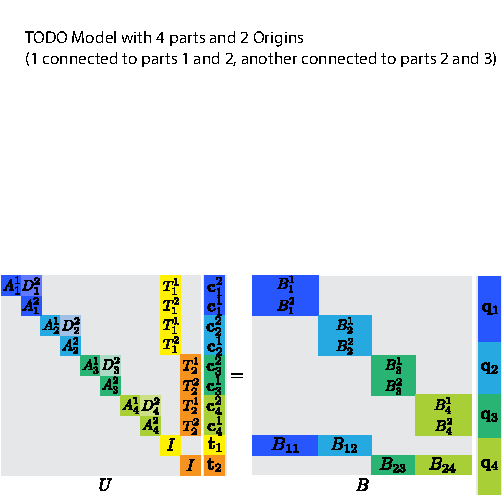
\includegraphics[width=\columnwidth]{figures/projection_operator_solve}
    \caption{A simple, four part model with two deformation origins and the corresponding matrix equation for the quadratic coefficients.}
    \label{fig:multiparts}
\end{figure}


Attempting to use $\Pmatxi$ in~\refeq{shapematch} on a per-part basis is problematic as it can become ill-posed, especially for planar boundary representations. 
To alleviate this problem we invoke the \emph{hierarchical ordering principle}, which argues that the behavior of a system is typically 
dominated by lower order effects~\cite{li2006regularities}. 
Mechanically, this principle suggests that the amount of motion modelled by increasingly high-order polynomials is decreasing. 
This implies that we can achieve acceptable shape matching results by performing shape matching hierarchically -- starting with the constant term and then 
fitting the remaining deformation with progressively higher-order deformations. 

For a given part, $\prt_i$, with associated origin $\bar{\refX}_j$ we first estimate the constant term, $\tr_i$ as the centroid of all parts associated with $\bar{X}_j$.
We next fit the linear part of the deformation by performing linear shape matching to $\prt_i$. 
This can be repeated for polynomials of arbitrary high order, for instance here we apply this approach to quadratic shape matching:

\begin{equation}
    \begin{split}
        \tr_i  & = \sum_{\prt_k \in \bar{\refX}_j} \underbrace{\mathbbm{1}^T\wt_k \samp{\Jnurbs}_k}_{B_{ik}}\vc{q}_k \\
        \vc{c}_i^1 & = \underbrace{\left(\samp{\Pmat^1}^T\wt_i\samp{\Pmat^1}\right)}_{A^1_i}^{-1}\bigg(\underbrace{\samp{\Pmat^1}^T\wt_i\samp{\Jnurbs}_i}_{B^1_i}\vc{q}_i-\underbrace{\samp{\Pmat^1}^T\wt_i\mathbbm{1}}_{T^1_i}\tr_i\bigg)\\
        \vc{c}_i^2 & = \underbrace{\left(\samp{\Pmat^2}^T\wt_i\samp{\Pmat^2}\right)}_{A^2_i}^{-1}\bigg(\underbrace{\samp{\Pmat^2}^T\wt_i\samp{\Jnurbs}_i}_{B^2_i}\vc{q}_i-\underbrace{\samp{\Pmat^2}^T\wt_i\samp{\Pmat^1}}_{D^2_i}\vc{c}_i^1 - \underbrace{\samp{\Pmat^2}^T\wt_i\mathbbm{1}}_{T^2_i}\tr_i\bigg)
    \end{split},
    \label{eq:hfit} 
\end{equation} where $\Pmat^l$ contains only the monomial basis of order $l$,  $\samp{\Pmat^1}$ is the stacked evaluation of this matrix at $n$ quadrature points and $\vc{c}^l_i$ are the corresponding coefficients. 
Finally, $\wt_i$ is the diagonal integration weight matrix and $\mathbbm{1}\in\real^{3n\times3}$ is a matrix of stacked $3\times3$ identity matrices -- one for each quadrature point.


%%single projector for every object
When assembled for all parts,~\refeq{hfit}, yields a block upper triangular matrix $U$ and a spare matrix $B$ ~(\reffig{multiparts}) which can be used to efficiently to compute the projection 
operator for the entire object $\Pi = U^{-1}B\vc{q}$. 
The structure of $U$ and $B$ ensures that $\Pi$ only couples objects which share deformation centers, which implies a sparse $\Pi$. 
The per-part projection operators $\Pi_i$ correspond to blocks of rows of $\Pi$. 
Coupling via the deformation origins ensures our method will reproduce rigid and linear deformations in regions around these points, while higher order 
terms help compensate for more local deformations.

\dave{should have done Chebyshev shape matching to ensure higher order terms are orthogonal which would gaurantee exact reconstruction}

\subsection{Meshless Blending Weight Computation}
\label{sec:weights}

\subsection{Choosing Deformation Centers}
\label{sec:origins}




%%%% OLD STUFF BELOW HERE  %%%%%
\subsection{Blending Weights}
\dave{Desireable Properties}
\dave{Construction via post normalization}
\dave{only need blending weights at quadrature points and surface samples so given sparse set of quadrature points compute blending weights using raycasting}
\dave{things to explain (1) raycasting works for overlapping geometric, seperated geometry (2) weights glue objects together}
\dave{maybe but weight figure here so reviewers immediately know that it looks pretty good}
All that remains for the deformation map is to compute blending weights. Our choice of the weighting function is guided by the simple idea that that for a given material point its weight should be highest to whichever surfaces it is closest. This idea lends itself to a simple distance-based weighting method. The first step in this process is to compute \textit{distance weights}. For a given point $\mathbf{X}$ and a set of $n$ we wish to compute a set of distance weights to each surface $\mathbf{\theta}(\mathbf{X}) = \left(\theta_1, \dots, \theta_i, \dots, \theta_n \right)$.

For the $i$-th surface, we first find the distance, $d_{\text{primary}}$, from the point $\mathbf{X}$ to the closest point, $\mathbf{p}$, on the surface. Next we wish to satisfy the condition that the distance weight is highest on the surface and it decays towards zero as it approaches other surfaces. To achieve this, we shoot a ray from $\mathbf{p}$ towards $\mathbf{X}$ and check for intersections between this ray and the other $n-1$ surfaces. If this ray hits another surface, we let $d_{\text{total}}$ be the distance from $\mathbf{p}$ to the closest ray hit $\mathbf{q}$. These two distances enable us to write a simple linear function to compute the \textit{distance weight}:
\begin{equation}
\theta_i = \max (1.0 - \frac{d_{\text{primary}}}{\min (d_{\text{total}}, D)}, 0.0)
\text{,}
\end{equation}
where $D$ is a fixed cutoff distance parameter. We see that this distance weight is the result of interpolating along this ray from $\mathbf{p}$ to $\mathbf{q}$ (or a fixed point that depends on $D$). Importantly, this gives a result where the distance weight to surface $i$ is equal to $1$ if it lies on $i$ and $0$ if it lies on another surface. More elaborate schemes may be developed for computing distances, such as using the Boundary Element Method, but we find this simple linear function to perform well for our purposes.

\begin{figure}
    \includegraphics[width=\columnwidth]{example-image-a}
    \caption{Figure showing how weight calculation works (left) ray casting plus result (right) after correcting for partition of unity}
    \label{fig:weightcompute}
\end{figure}

Now that we have a set of distances weights $\mathbf{theta}$, we seek to form a final set of \textit{blending weights} $\mathbf{w}(\mathbf{X}) =  \left( w_1, \dots, w_i, \dots, w_n \right)$ to blend the polynomials of the $n$ shape elements. In constructing these blending weights, we require that they adhere to a set of conditions. We require that (1) each weight is non-negative, (2) the sum of the weights is equal to 1 (\textit{partition of unity}), (3) and that if a point lies on a surface $i$, it will have a weight of 1 to $i$ and consequently zero to the others. To produce these blending weights we form a quadratic program that satisfies these constraints:
\begin{equation}
\begin{aligned}
\mathbf{w}(\mathbf{X}) = \min_{\mathbf{w}} \quad & \mathbf{w}^T \Theta(\mathbf{X}) \mathbf{w}    \\
\textrm{s.t.} \quad & 0 \leq w_i \leq 1                     \\
                    &   \sum_i^n w_i = 1                      \\
\end{aligned}
\end{equation}

where
\begin{equation}
     \Theta(\mathbf{X}) = \text{diag}\left( \frac{1}{\theta_1},\frac{1}{\theta_2},\dots,\frac{1}{\theta_n}\right)
\end{equation}
We see that through the use of linear constraints we satisfy conditions (1) and (2). Satisfying the third condition (3) is achieved through using the distance weights. Intuitively, we see that for some small $\theta_i$, $\frac{1}{\theta_i}$ will be very large, encouraging the quadratic program to assign a small weight for $w_i$. Conversely, we see the opposite effect for large values of $\theta_i$.

\subsection{Multiple Part Projection}
\dave{explain why you need to share constant terms (fit polynomial around a point in space), explain clustering and how to pick, forward reference to quadrature point}
\subsection{Quadrature Points}
\dave{quadrature via raycasting}
The last step before we may discuss the dynamic simulation is to describe our strategy for generating material points $\mathbf{X}$ in the undeformed model. Our volume integration strategy is based on \cite{KHOSRAVIFARD201030} which we briefly describe in the following section

This paper addresses the integration of volume integrals of the form $\mathbf{I} = \int_\Omega f(\mathbf{x}) d\Omega$ where $\mathbf{x} = (x_1,x_2,x_3)$. The authors show that through application of the Green-Gauss theorem, this integral may be rewritten as 2D integral over a $yz$ plane where at each position along the plane we evaluate a line integral along the $x$-axis. To evaluate these line integrals, a raycasting procedure is performed to find a set of intersection along the line. These intersection define integration domains in which we sample 3D integration points. As a result of integrating over the 2D plane and raycasting at each 2D point, we produce an integration rule over the entire domain that can converge to the true integral value.

In our approach we modify the raycasting procedure by allowing integration over intersecting NURBS surfaces. It is common in NURBS modeling to produce models in which many surfaces overlap. To account for this we augment the raycasting intersection step to use an approach common in Constructive Solid Geometry (CSG). For the set of intersection intervals, we instead take the union over all intervals to yield a new set of intervals handling intersecting solids. We find that this extension serves as a simple and practical approach to support inexact models (\myworries{not sure what to right here}). We note that this solution is not perfect and making this intersection step more robust serves as future work.

\begin{figure}
    \includegraphics[width=\columnwidth]{example-image-a}
    \caption{Figure showing how raycasting quadrature works (top), convergence plot for volume integration (bottom}
    \label{fig:raycasting}
\end{figure}

\subsection{Mass Matrix}
The kinetic energy for a model may be expressed as
\begin{equation}
T = \frac{1}{2}\int_{ \Omega} \rho \dot{\mathbf{x}}^T\dot{\mathbf{x}} d\Omega
\text{,}
\end{equation}
where $\Omega$ is the 3D integration domain, $\rho$ is the density, and $\dot{\mathbf{x}}$ is the velocity for some point in the domain. Using the deformation map defined in \ref{eqn:compact_x_map}, we may rewrite this kinetic energy as
\begin{equation}
\begin{split}
T & = \frac{1}{2}\int_{ \Omega} \rho \dot{\mathbf{q}}^T \mathbf{J}^T\mathbf{Y(X)}^T\mathbf{Y(X)}\ d\Omega \\
  & = \frac{1}{2} \dot{\mathbf{q}}^T \mathbf{J}^T \left[ \int_{ \Omega} \rho \mathbf{Y(X)}^T\mathbf{Y(X)} d\Omega \right] \mathbf{J}\dot{\mathbf{q}} \\
  & = \frac{1}{2} \dot{\mathbf{q}}^T \mathbf{M} \dot{\mathbf{q}}
\end{split}
\text{.}
\end{equation}
The second line is a result of the fact that all terms except for $\mathbf{Y(X)}$ are spatially constant, allowing us to move these outside the volume integral, which enables fast assembly of the mass matrix, $\mathbf{M}$.
\subsection{Error Energy}
Over the course of the simulation we may see the true boundary values deviate from their positions estimated by the polynomial. This is most notable in cases where the degree of the polynomial on a NURBS is higher than the degree of the B-spline surface. To address this we augment our kinetic energy with a term to account for this error. The error for a boundary point $\mathbf{x}_i^*$ that is known to lie on the limit surface of the NURBS can be written as
\begin{equation}
\begin{split}
\epsilon_i & = ||\mathbf{x}(\mathbf{X}_i) - \mathbf{x}_i^*|| \\
		   & = ||(\mathbf{Y}(\mathbf{X}_i)\mathbf{L} - \mathbf{S_i})\mathbf{\hat{b}}||
\end{split}
\text{,}
\end{equation}
where $\mathbf{S_i}$ extracts $\mathbf{x}_i^*$ from $\mathbf{\hat{b}}$. We modify this error further to be expressed in terms of the control points. We note that $\mathbf{x}^*(u,v)$ yields the position on the NURBS surface whereas $\mathbf{x(X)}$ is the deformed value estimated by the polynomial fitting. Furthermore $\mathbf{X}$ may be written as a function of the parametric coordinates $\mathbf{X}(u,v)$ as its position on the surface is produced using the initial set of control points representing the undeformed model. This leads to an energy potential over the NURBS surface in parametric space
\begin{equation}
T_E = \iint (\mathbf{x}(\mathbf{X}(u,v)) - \mathbf{x}^*(u,v))^T(\mathbf{x}(\mathbf{X}(u,v)) - \mathbf{x}^*(u,v)) du dv
\text{.}
\end{equation}
The discrete form of this written in terms of the control points may be written as
\begin{equation}
\begin{split}
T_E & = \sum_i^N  \dot{\mathbf{q}}^T\mathbf{J}^T(\mathbf{Y}(\mathbf{X}_i)\mathbf{L} - \mathbf{S_i})^T(\mathbf{Y}(\mathbf{X}_i)\mathbf{L} - \mathbf{S_i})\mathbf{J}\dot{\mathbf{q}} \\
  & = \dot{\mathbf{q}}^T\mathbf{J}^T \left[ \sum_i^N  (\mathbf{Y}(\mathbf{X}_i)\mathbf{L} - \mathbf{S_i})^T(\mathbf{Y}(\mathbf{X}_i)\mathbf{L} - \mathbf{S_i}) \right] \mathbf{J}\dot{\mathbf{q}} \\
  & = \dot{\mathbf{q}}^T \mathbf{M}_E \dot{\mathbf{q}}
\end{split}
\text{,}
\end{equation}
where $N$ is the total number of boundary points and $\mathbf{M}_E$ is our \textit{error mass matrix}.
% \subsection{Generalized Forces}
% We write our potential energy as 
% \begin{equation}
%     V = \int_\Omega \psi(\mathbf{F(X)}) d\Omega
% \text{.}
% \end{equation}
% To evaluate this energy (as well as its derivatives), we require a definition for the deformation gradient, $\mathbf{F(X)}$:
% \begin{equation}
%         \mathbf{F(X)} = \frac{\partial \mathbf{x}}{\partial \mathbf{X}}
%                = \frac{\partial \mathbf{Y(X)}}{\partial \mathbf{X}}\mathbf{L}\hat{\mathbf{b}}
% \text{.}
% \end{equation}
% In the expression for the deformed position $\mathbf{x(X)}$ we see that the dependence on $\mathbf{X}$ only exists in $\mathbf{Y(X)}$, making $\mathbf{L}$ and $\hat{\mathbf{b}}$ constant terms when compute $\mathbf{F}$. Full details on how to compute $\mathbf{F}$ and its derivative $\frac{\partial \mathbf{F}}{\partial \mathbf{q}}$ may be found in the appendix. (\myworries{I just wrote this because I'm too tired to right the d etails right now :p}. Now that we have an expression for the deformation gradient, we discretize our potential energy as follows
% \begin{equation}
%     V =  \sum_i^m \psi(\mathbf{F(X}_i) A_i
% \text{,}
% \end{equation}
% where $m$ is the number of integration points and $A_i$ is the volume for the $i$-th integration point.

% Like in the case of the kinetic energy, we also introduce an error force potential, which takes the simple form
% \begin{equation}
% V_E = \mathbf{q}^T \mathbf{M}_E \mathbf{q}
% \end{equation}
\subsection{Deformation Gradient}
At this point we have shown how to fit a polynomial describing the deformation of each surface. With these polynomial coefficients coupled with their associated centers of mass, we can construct an estimate of some arbitrary material point $\mathbf{X}$ using the deformation described by the surface. This lends itself to a general definition for the deformed position of a point as a weighted sum of the polynomials, which yields a unique polynomial for the point. Thus we arrive at a definition for the deformed position, $\mathbf{x}$, of a material point $\mathbf{X}$ in the undeformed space:
\begin{equation}
\label{eqn:deformation_map}
	\mathbf{x}(\mathbf{X}) = \sum_i^n w_i(\mathbf{X}) \left[ \mathbf{M}(\mathbf{X-\bar{X}}_j)\mathbf{c}_i + \mathbf{t}_j \right]
	\text{,}
\end{equation}
where we have $n$ surfaces, and $w_i$ and $\mathbf{c}_i$ are the weights and the coefficients for the $i$-th surface, respectively. The terms $\mathbf{\bar{X}}_j$ and $\mathbf{t}_j$ the undeformed and deformed centers of mass, respectively, that are associated with the $i$-th surface.


\subsection{External Forces}
\subsection{Time Integration}
With our definition of the deformation map as well as a strategy for integrating the volume, we now have the necessary ingredient to perform dynamic simulation. We follow the Variational Mechanics approach that defines a pair of kinetic and potential energies, and we apply the Euler-Lagrange equation to develop our equations of motion.

Before we define these energies we first would like to simplify the form of the deformation map presented in equation \ref{eqn:deformation_map}. We may write $\mathbf{x}(\mathbf{X})$ in matrix form as
\begin{equation}
\mathbf{x}(\mathbf{X}) = \underbrace{\left[w_1\mathbf{M}(\mathbf{X - \bar{X}}_j) \dots w_n\mathbf{M}(\mathbf{X - \bar{X}}_j) \middle| \sum_i^{n_1}w_1^i\mathbf{I} \dots \sum_i^{n_m}w_m^i\mathbf{I} \right]}_{\mathbf{Y}(\mathbf{X})}
\begin{bmatrix}
\mathbf{\hat{c}} \\
\mathbf{\hat{t}}
\end{bmatrix}
\text{,}
\end{equation}
\myworries{I'm not sure how to write this matrix form for x(X), especially on finding the best notation for the center of mass indexing. So this above equation is temporary.}
where we have $n$ shape elements, $m$ centers of mass. We simplify the above equation and use the following form
\begin{equation}
\label{eqn:x_simple_form}
\mathbf{x}(\mathbf{X}) = \mathbf{Y}(\mathbf{X})\mathbf{L}\hat{\mathbf{b}}
\text{,}
\end{equation}
where we make use of equation \ref{eqn:c_multiple_elements} to rewrite this in terms of the boundary points $\mathbf{\hat{b}}$. As one final step, we rewrite this again in terms of the control points of our NURBS surfaces:
\begin{equation}
\label{eqn:compact_x_map}
\mathbf{x}(\mathbf{X}) = \mathbf{Y}(\mathbf{X})\mathbf{LJq}
\text{,}
\end{equation}
where we use the fact that $\mathbf{\hat{b}} = \mathbf{Jq}$. \myworries{not a fan of this, perhaps we change $\hat{b}$ to something else...} This gives us an expression for the deformed position in terms of our generalized coordinates, $\mathbf{q}$.

\dave{discrete Equations of motion with quadratured integrals, reference/details on how we handle collisions}

We have now provided all the necessary ingredient to produce equations of motion for deformable bodies, which we derive via Euler-Lagrange equation. We begin with the Lagrangian
\begin{equation}
    L=(T+T_E)-(V + V_E)
\end{equation}
Then from the Euler-Lagrange equation we have:
\begin{equation}
    \frac{d}{dt} \frac{\partial L}{\partial \dot{\mathbf{p}}} + \frac{\partial L}{\partial {\mathbf{p}}} = 0
\end{equation}
\myworries{todo: not totally sure what to write here since we're experimenting with both linearly implicit backward euler as well as Newton's method soon}



\begin{equation}
   \frac{\partial L}{\partial \mathbf{q}} = \sum_i^m \frac{\partial V_i}{\partial \mathbf{q}} = \sum_i^m \frac{\partial \psi(\mathbf{F_i)}}{\partial \mathbf{F}}\frac{\partial \mathbf{F_i}}{\partial \mathbf{q}}A_i
\end{equation}
\


%%% ------- OLD STUFF BELOW --------
% \section{Methods}
% \dave{We should probably put some pseudo code for the preprocessing and the runtime algorithms right up fron, along with a quick textual walk through of the method.}
% Given a volumetric model composed of one or more NURBS surfaces, the surface of each surface is reconstructed using a set of control points $\textbf{p}$ and their associated weights $w$. Following D-NURBS \cite{10.1145/176579.176580}, we take our degrees of freedom (DOF) to be control points of the surfaces and produce displacements directly on these control points at each simulation step. We note that we used a simplified version of D-NURBS in which the weights are held constant throughout the simulation and find this not to be limiting \myworries{(feel like we'll need better justification than saying just this?)}. We represent the degrees of freedom for the $i$-th NURBS surface with $m$ control points as $\mathbf{q}_i = \left[ \mathbf{p}_1^T, \dots, \mathbf{p}_m^T \right]^T \in \mathbb{R}^{3m}$. From this definition, we write the DOF for the entire model as $\mathbf{q} = \left[ \mathbf{q}_i^T, \dots, \mathbf{q}_n^T \right]^T$ where $n$ is the number of NURBS surfaces for the model. 

% To evaluate the volumetric integrals in solid mechanics models, we require material points $\mathbf{X} \in \mathbb{R}^{3m}$ in the undeformed space that serve as integration points. Our shape matching element method enables us to evaluate the deformed positions of the material points strictly using positions defined on the boundary. Like in VEM, we fit a polynomial to each boundary primitive (NURBS in this case) describing its deformation. The fitting of these polynomials closely follows that of the Shape Matching \cite{10.1145/1073204.1073216} approach where we perform a least squares polynomial fit to the deformed boundary points. These boundary points are represented by sampled positions on each NURBS surface. Since each surface is associated with a single polynomial, we can construct a unique polynomial for some arbitrary point by blending these polynomials. Thus given some material point $\mathbf{X}_i$ we find it's corresponding deformed position $\mathbf{x}_i$ via a weighted combination of the polynomials. This permits us to build a general deformation map which we use to construct our equations of motion.

% In the following sections, we will first review the simplified D-NURBS model used to form our generalized coordinates. We then present our shape matching algorithm for fitting polynomials to surfaces .... In section ... we next describe how to blend these surface polynomials to construct a general deformation map for material points. Section ... describes our strategy for selecting integration points in the volume through a raycasting approach. Finally, we formulate our equations of motions from a Lagrangian formulation.

% \section{D-NURBS Model}
% \myworries{TODO: Most of these matrices should be paranthesis matrices}
% We provide a brief overview of the D-NURBS formulation presented in \cite{10.1145/176579.176580}. Our models in our method are composed of a collection of NURBS surfaces. 

% \subsection{D-NURBS Formulation}
% A point on a NURBS surface is typically expressed in the following form
% \begin{equation}
% \label{eqn:nurbs_srf}
%     \mathbf{x}(u,v) = \frac{\sum_{i=1}^{n}\sum_{j=1}^{m}  \mathbf{p}_{i,j} w_{i,j} B_{i,k}(u)B_{j,l}(v)}
%     {\sum_{i=1}^{n}\sum_{j=1}^{m} w_{i,j} B_{i,k}(u)B_{j,l}(v)}
%     \text{,}
% \end{equation}
% where where have a total of $nm$ control points $\mathbf{p}$ and weights $w$. Using the B-spline basis functions and the weighted control points, this formula gives a map from our parametric coordinates $u,v$ to their corresponding position on the surface in $\mathbb{R}^{3m}$. $B_{i,k}(u)$ is the B-spline basis function for the $i-th$ control point with degree $k-1$.

% We would like our generalized coordinates to be the control points of the model so that the dynamics operates directly on the original representation. Therefore, we would like to rewrite equation \ref{eqn:nurbs_srf} in the form
% \begin{equation}
%     \mathbf{x}(u,v) = \mathbf{J}(u,v)\mathbf{q}
%     \text{,}
% \end{equation}
% where $\mathbf{q} = \left[ \mathbf{p}_{1,1}^T, \dots, \mathbf{p}_{i,j}^T, \dots, \mathbf{p}_{n,m}^T \right]^T \in \mathbb{R}^{3nm}$ is the set of $nm$ control points \myworries{in the overview I just write $n$ control points, but here i'm writing $nm$} for a single NURBS surface arranged as a column vector. $\mathbf{J} \in  \mathbb{R}^{3 x 3nm}$ is the NURBS jacobian that maps $(u,v)$ coordinates to world positions in $\mathbb{R}^{3}$.

% The NURBS jacobian, $\mathbf{J}$, is a matrix composed of horizontally concatenated $3x3$ blocks where the $(i,j)$-th block is $\frac{\partial \mathbf{x}}{\partial \mathbf{p}_{i,j}}$ for the $(i,j)$-th control point. $\frac{\partial \mathbf{x}}{\partial \mathbf{p}_{i,j}}$ is a diagonal $3x3$ matrix where each diagonal entry $N_{i,j}(\mathbf{u})$ takes the form

% \begin{equation}
% \label{eqn:jacobian_diagonal}
%     N_{i,j}(u,v)
%     = \frac{w_{i,j} B_{i,k}(u)B_{j,l}(v)}{\sum_{i=1}^{n}\sum_{j=1}^{m} w_{i,j} B_{i,k}(u)B_{j,l}(v)}
%     \text{.}
% \end{equation}
% Thus the NURBS jacobian for a single $(u,v)$ pair is written as
% \begin{equation}
% \label{eqn:uv_jacobian}
%     \mathbf{J}(u,v) =
%     \left[ \frac{\partial \mathbf{x}}{\partial \mathbf{p}_{1,1}} \dots
%            \frac{\partial \mathbf{x}}{\partial \mathbf{p}_{i,j}} \dots 
%            \frac{\partial \mathbf{x}}{\partial \mathbf{p}_{n,m}}
%     \right]
%     \text{.}
% \end{equation}

% This formulation is a simplification of the full D-NURBS described in \cite{10.1145/176579.176580} the weights of the NURBS are fixed throughout the simulation. Permitting the dynamics to modify weights would likely improve the expressiveness of the kinematics, but we find fixing the weights affords sufficiently expressive results and improves performance. The performance improvement is a result of having fixed $N_{i,j}(u,v)$ entries over the course of the simulation. The full D-NURBS model requires rebuilding the jacobian and consequently the mass matrices at each time step. 

% \subsection{Generalized Coordinates for a NURBS model}
% The above formulation describes developing the map from a single $(u,v)$ coordinate to its corresponding position on the surface. In our simulation we represent the entire boundary of the NURBS model, so we require samples along each surface. We emphasize that we only require an initial selection of $(u,v)$ coordinates across each surface and the dynamics of the simulation modifies the set of control points $\mathbf{q}$ to modify the world space maps $\mathbf{x}(u,v)=\mathbf{J}(u,v)\mathbf{q}$.

% Let's say for a NURBS surface on the model the DOF column vector is $\mathbf{q}_i$, which is the subset of control points in the generalized coordinates for the $i$-th surface. For a given surface with $m$ pairs of $\mathbf{u}=(u,v)$ coordinates sampled in parametric space, we write the jacobian for the $i$-th surface as \myworries{(should I use something like $\hat{\mathbf{J}}$ instead?)}
% \begin{equation}
% \label{eqn:surface_jacobian}
%     \mathbf{J}_i =
%     \left[ \mathbf{J}(\mathbf{u})_1^T \dots \mathbf{J}(\mathbf{u})_m^T \right]^T
%     \text{.}
% \end{equation}
% Then if $\mathbf{x}_i$ is the set of $m$ world space positions for the $i$-th surface, we may write $\mathbf{x}_i = \mathbf{J}_i \mathbf{q}_i$. Finally, given the full set of generalized coordinates $\mathbf{q} = \left[ \mathbf{q}_i^T, \dots, \mathbf{q}_n^T \right]^T$ with $n$ surfaces, we may write jacobian $\mathbf{J}$ for the entire model as a block diagonal matrix:
% \begin{equation}
% \mathbf{J} = \left[ \begin{array}{ccccc}
% \mathbf{J}_1 &  &  &  &  \\
%  & \ddots &  &  &  \\
%  &  & \mathbf{J}_i & &  \\
%  &  &  & \ddots &  \\
%  &  &  &  & \mathbf{J}_n \\
% \end{array} \right]
% \text{.}
% \end{equation}
% With this equation, the full set of world positions of the NURBS model may be written as $\mathbf{x} = \mathbf{J}\mathbf{q} \in \mathbb{R}^{3N}$ where $N$ is the total number of $(u,v)$ coordinates.


% \subsection{Shape Matching with Multiple Elements}

% \subsection{Computing the Blending Weights}


% \subsection{Generalized Inertia}



% \subsection{Time Integration}
% 